
\lecture{Deadlock (impasse)}{deadlock}

\frame{\title{\insertlecture}\maketitle}

\section{\insertlecture}
\begin{frame}{\insertlecture}
  \def\A{{\color{brown}A}}
  \def\B{{\color{blue}B}}
  \def\dist{15mm}
  \def\waiting{{\color{red} esperando...}}
    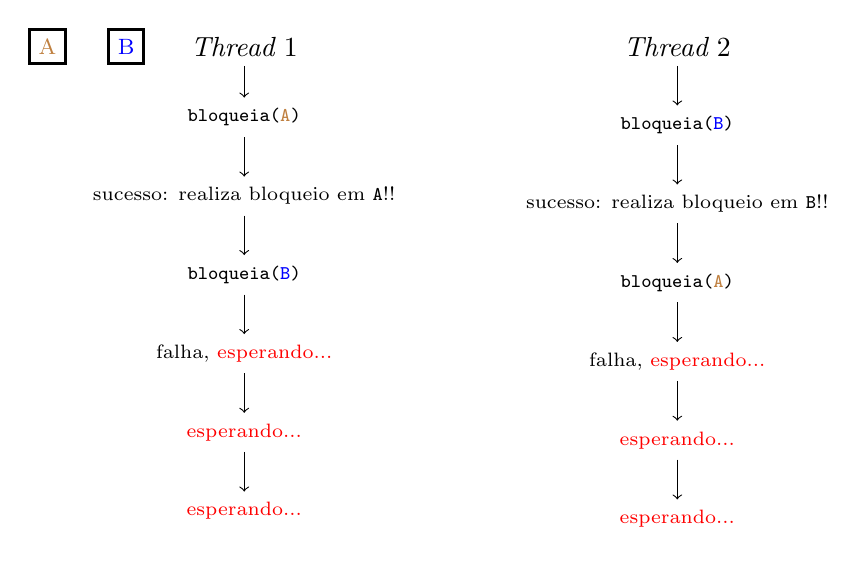
\begin{tikzpicture}[memory/.style={rectangle,draw,very thick,anchor=east,font=\footnotesize},
    op/.style={rectangle,very thick,font=\scriptsize}]
    \node (mem1) [memory] {\A};
    \node (mem2) [memory, right of=mem1] {\B};

    \node (t1) [right of=mem1,xshift=\dist] {{\em Thread} $1$};
    \node (t1op1) [below of=t1,op,yshift=1mm] {{\tt bloqueia(\A)}};
    \node (t1op2) [below of=t1op1,op] {sucesso: realiza bloqueio em
{\tt A}!!};
    \node (t1op3) [below of=t1op2,op] {{\tt bloqueia(\B)}};
    \node (t1op4) [below of=t1op3,op] { falha, \waiting};
    \node (t1op5) [below of=t1op4,op] {\waiting};
    \node (t1op6) [below of=t1op5,op] {\waiting};

    \node (t2) [right of=t1, xshift=3*\dist] {{\em Thread} $2$};
    \node (t2op1) [below of=t2,op] {{\tt bloqueia(\B)}};
    \node (t2op2) [below of=t2op1,op] {sucesso: realiza bloqueio em
{\tt B}!!};
    \node (t2op3) [below of=t2op2,op] {{\tt bloqueia(\A)}};;
    \node (t2op4) [below of=t2op3,op] {falha, {\color{red} esperando...}};
    \node (t2op5) [below of=t2op4,op] {\waiting};
    \node (t2op6) [below of=t2op5,op] {\waiting};

    \path (t1) edge[->] (t1op1);
    \path (t1op1) edge[->] (t1op2);
    \path (t1op2) edge[->] (t1op3);
    \path (t1op3) edge[->] (t1op4);
    \path (t1op4) edge[->] (t1op5);
    \path (t1op5) edge[->] (t1op6);

    \path (t2) edge[->] (t2op1);
    \path (t2op1) edge[->] (t2op2);
    \path (t2op2) edge[->] (t2op3);
    \path (t2op3) edge[->] (t2op4);
    \path (t2op4) edge[->] (t2op5);
    \path (t2op5) edge[->] (t2op6);
  \end{tikzpicture}

\end{frame}

\begin{frame}[fragile]{Exemplo de código com possível deadlock}
\lstset{emph={MUTEX1},emphstyle={\color{blue}},
emph={[2]mutex0},emphstyle={[2]\color{red}},
language=C,basicstyle=\scriptsize}  

\begin{lstlisting}
  mutex_t mutex0, MUTEX1;
\end{lstlisting}

\lstset{frame=single}
\begin{columns}
    \begin{column}{.5\textwidth}
      \begin{block}{Thread 0}
      \begin{lstlisting}
        mutex_lock(&mutex0);
        mutex_lock(&MUTEX1);
        /**
        * região crítica
        */
        mutex_unlock(&MUTEX1);
        mutex_unlock(&mutex0);
      \end{lstlisting}
    \end{block}
  \end{column}
  \begin{column}{.5\textwidth}
    \begin{block}{Thread 1}
      \begin{lstlisting}
        mutex_lock(&MUTEX1);
        mutex_lock(&mutex0);
        /**
        * região crítica
        */
        mutex_unlock(&mutex0);
        mutex_unlock(&MUTEX1);
      \end{lstlisting}
    \end{block}
  \end{column}
\end{columns}


\end{frame}

\begin{frame}{Grafo de alocação de recursos}
  
  \begin{columns}

    \begin{column}{0.5\textwidth}


      {\footnotesize P -- processo \\ R -- recurso \\ A -- arcos \\
        $P\rightarrow R$, processo $P$ requisita recurso $R$\\
        $R\rightarrow P$, recurso $R$ é atribuído para $P$\bigskip}

      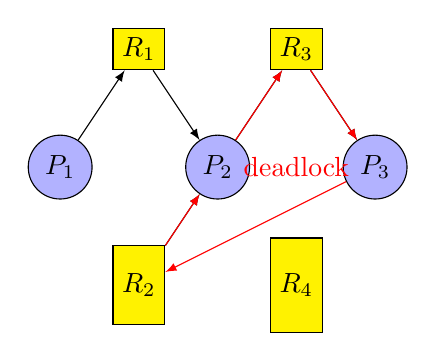
\begin{tikzpicture}
        \tikzset{proc/.style={circle,draw,fill=white!70!blue},
          res/.style={rectangle,draw,fill=yellow}}

        \foreach \x in {1,2,3}
        \node[proc] (p\x) at (2*\x,0) {$P_\x$};
        \foreach \x in {1,3}
        \node[res] (r\x) at (2+\x,1.5) {$R_\x$};
        \node[res,minimum height=1cm] (r2) at (3,-1.5) {$R_2$};
        \node[res,minimum height=1.2cm] (r4) at (5,-1.5) {$R_4$};

        \draw[->,>=latex] (p1) -- (r1);
        \draw<1>[->,>=latex] (p2) -- (r3);
        \draw<2>[->,>=latex,color=red] (p2) -- (r3);
        \draw[->,>=latex] (r1) -- (p2);
        \draw<1>[->,>=latex] (r2) -- (p2);
        \draw<2>[->,>=latex,color=red] (r2) -- (p2);
        \draw<1>[->,>=latex] (r3) -- (p3);
        \draw<2>[->,>=latex,color=red] (r3) -- (p3);
        \draw<2>[->,>=latex,color=red] (p3) -- (r2);

        \node<2>[color=red] at (5,0) {deadlock};

      \end{tikzpicture}

      \end{column}
      \begin{column}{0.35\textwidth}
              Representação\\

        \small
        \begin{tabbing}
        $P =$ \= $\{P_1, P_2, P_3\}$\\
        $R =$ \> $\{R_1, R_2, R_3, R_4\}$\\
        $\vec{A} =$ \> $\{$\=$\{P_1,R_1\}, \{P_2, R_3\},$ \\
        \>\> $\{R_1,P_2\}, \{R_2,P_2\},$ \\
        \>\> $\{R_2,P_1\}, \{R_3,P_3\}$\only<2>{$,$}\only<1>{$\}$}\\
        \>\> \only<2>{{\color{red}$\{P_3,R_2\}\}$}}\\
      \end{tabbing}
      Se um grafo não tiver ciclo não possui {\em deadlock}.
    \end{column}

  \end{columns}

\end{frame}



%\ifnum1=2%%%%%%%%%%%%%%%%%%%%%%%%%%%%%%%%BUFFER

\begin{frame}{Grafo de alocação com ciclo}{Vários recursos}
  \small
  Um ciclo pode ser eliminado com a liberação de um recurso e o {\em deadlock} é desfeito.

  \begin{center}
        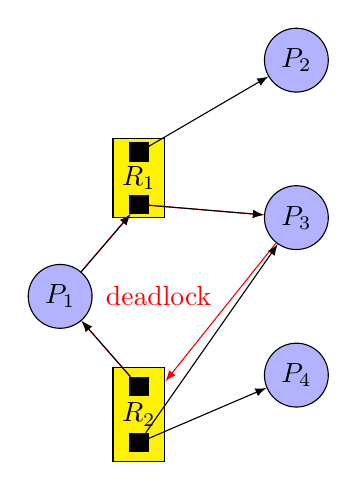
\begin{tikzpicture}
        \tikzset{proc/.style={circle,draw,fill=white!70!blue},
          res/.style={rectangle,draw,fill=yellow}}


        \node[proc] (p1) at (0,0) {$P_1$};
        \node[proc] (p2) at (3,3) {$P_2$};
        \node[proc] (p3) at (3,1) {$P_3$};
        \node[proc] (p4) at (3,-1) {$P_4$};
        \node[res,minimum height=1cm] (r1) at (1,1.5) {$R_1$};
        \node[res,minimum height=1.2cm] (r2) at (1,-1.5) {$R_2$};
        \node[fill,draw] (R11) at (r1.north)[yshift=-.175cm] {};
        \node[fill,draw] (R12) at (r1.south)[yshift=.175cm] {};
        \node[fill,draw] (R21) at (r2.north)[yshift=-.25cm] {};
        \node[fill,draw] (R22) at (r2.south)[yshift=.25cm] {};

        \draw<1>[->,>=latex,color=red] (p1) -- (R12);
        \draw<2>[->,>=latex] (p1) -- (R12);
        \draw[->,>=latex] (R11) -- (p2);
        \draw<1>[->,>=latex,color=red] (R21) -- (p1);
        \draw<2>[->,>=latex] (R21) -- (p1);
        \draw<1>[->,>=latex,color=red] (R12) -- (p3);
        \draw<2>[->,>=latex] (R12) -- (p3);
        \draw<1>[->,>=latex,color=red] (p3) -- (r2);
        \draw<2>[->,>=latex] (R22) -- (p3);

        \draw<1>[->,>=latex] (R22) -- (p4);

        \node<1>[color=red] at (1.25,0) {deadlock};

      \end{tikzpicture}
    \end{center}
    \only<2>{Quando $P_4$ libera o recurso acaba o {\em deadlock}}

\end{frame}

\begin{frame}{Solução para recursos com N objetos cada}

  \begin{itemize}
  \item Algoritmo do banqueiro (Dijkstra)
  \end{itemize}
  
\end{frame}

\begin{frame}{$+$Sincronização}
  \begin{itemize}
  \item Jantar dos filósofos;
  \item Monitores;
  \item Algoritmo do banqueiro.
  \end{itemize}

\end{frame}

%\fi
